% !TeX spellcheck = de_DE
% !TeX encoding = utf8

%Die Angabe des schlauen Spruchs auf diesem Wege funtioniert nur,
%wenn keine Änderung des Kapitels mittels den in preambel/chapterheads.tex
%vorgeschlagenen Möglichkeiten durchgeführt wurde.
\setchapterpreamble[u]{%
  \dictum[Albert Einstein]{Probleme kann man niemals mit derselben Denkweise lösen, durch die sie entstanden sind.}
}
\chapter{LaTeX-Tipps}
\label{chap:latextipps}

Pro Satz eine neue Zeile.
Das ist wichtig, um sauber versionieren zu können.
In LaTeX werden Absätze durch eine Leerzeile getrennt.

Folglich werden neue Abstäze insbesondere \emph{nicht} durch Doppelbackslashes erzeugt.
Beispielsweise begann der letzte Satz in einem neuen Absatz.
Eine ausführliche Motivation hierfür findet sich in \url{http://loopspace.mathforge.org/HowDidIDoThat/TeX/VCS/#section.3}.

\section{File-Encoding und Unterstützung von Umlauten}
\label{sec:firstsectioninlatexhints}
Die Vorlage wurde 2010 auf UTF-8 umgestellt.
Alle neueren Editoren sollten damit keine Schwierigkeiten haben.

\section{Zitate}
Referenzen werden mittels \texttt{\textbackslash cite[key]} gesetzt.
Beispiel: \cite{WSPA} oder mit Autorenangabe: \citet{WSPA}.

Der folgende Satz demonstriert \begin{inparaenum}[1.]
  \item die Großschreibung von Autorennamen am Satzanfang,
  \item die richtige Zitation unter Verwendung von Autorennamen und der Referenz,
  \item dass die Autorennamen ein Hyperlink auf das Literaturverzeichnis sind sowie
  \item dass in dem Literaturverzeichnis der Namenspräfix \enquote{van der} von \enquote{Wil M.\,P.\ van der Aalst} steht.
\end{inparaenum}
\Citet{RVvdA2016} präsentieren eine Studie über die Effektivität von Workflow-Management-Systemen.

Der folgende Satz demonstriert, dass man mittels \texttt{label} in einem Bibliopgrahie"=Eintrag den Textteil des generierten Labels überschreiben kann, aber das Jahr und die Eindeutigkeit noch von biber generiert wird.
Die Apache ODE Engine \cite{ApacheODE} ist eine Workflow-Maschine, die BPEL-Prozesse zuverlässig ausführt.

Wörter am besten mittels \texttt{\textbackslash enquote\{...\}} \enquote{einschließen}, dann werden die richtigen Anführungszeichen verwendet.

Beim Erstellen der Bibtex-Datei wird empfohlen darauf zu achten, dass die DOI aufgeführt wird.

\section{Mathematische Formeln}
\label{sec:mf}
Mathematische Formeln kann man $so$ setzen. \texttt{symbols-a4.pdf} (zu finden auf \url{http://www.ctan.org/tex-archive/info/symbols/comprehensive/symbols-a4.pdf}) enthält eine Liste der unter LaTeX direkt verfügbaren Symbole.
Z.\,B.\ $\mathbb{N}$ für die Menge der natürlichen Zahlen.
Für eine vollständige Dokumentation für mathematischen Formelsatz sollte die Dokumentation zu \texttt{amsmath}, \url{ftp://ftp.ams.org/pub/tex/doc/amsmath/} gelesen werden.

Folgende Gleichung erhält keine Nummer, da \texttt{\textbackslash equation*} verwendet wurde.
\begin{equation*}
  x = y
\end{equation*}

Die Gleichung~\ref{eq:test} erhält eine Nummer:
\begin{equation}
  \label{eq:test}
  x = y
\end{equation}

Eine ausführliche Anleitung zum Mathematikmodus von LaTeX findet sich in \url{http://www.ctan.org/tex-archive/help/Catalogue/entries/voss-mathmode.html}.

\section{Quellcode}
\Cref{lst:ListingANDlstlisting,helloworld} zeigen, wie man Programmlistings einbindet.
Mittels \texttt{\textbackslash lstinputlisting} kann man den Inhalt direkt aus Dateien lesen.

%Listing-Umgebung wurde durch \newfloat{Listing} definiert
\begin{Listing}
  \begin{lstlisting}[language=XML]
<listing name="second sample">
  <!-- comment -->
  <content>not interesting</content>
</listing>
\end{lstlisting}
  \caption{lstlisting in einer Listings-Umgebung, damit das Listing durch Balken abgetrennt ist}
  \label{lst:ListingANDlstlisting}
\end{Listing}

%TODO: Currently not shown in TOC
\lstinputlisting[language=C++,label=helloworld,caption={"`hello world"' in C++.},float]{code/helloworld.cpp}

Quellcode im \lstinline|<listing />| ist auch möglich.

\section{Abbildungen}

Die \cref{fig:chor1} und \ref{fig:chor2} sind für das Verständnis dieses Dokuments wichtig.
Im Anhang zeigt \vref{fig:AnhangsChor} erneut die komplette Choreographie.

%Die Parameter in eckigen Klammern sind optionale Parameter - z.B. [htb!]
%htb! bedeutet: "Liebes LaTeX, bitte platziere diese Abbildung zuerst hier ("_h_ere"). Falls das nicht funktioniert, dann bitte oben auf der Seite ("_t_op"). Und falls das nicht geht, bitte unten auf der Seite ("_b_ottom"). Und bitte, bitte bevorzuge hier und oben, auch wenn's net so optimal aussieht ("!")
%Diese sollten nach Möglichkeit NICHT verwendet werden. LaTeX's Algorithmus für das Platzieren der Gleitumgebung ist schon sehr gut!
\begin{figure}
  \centering
  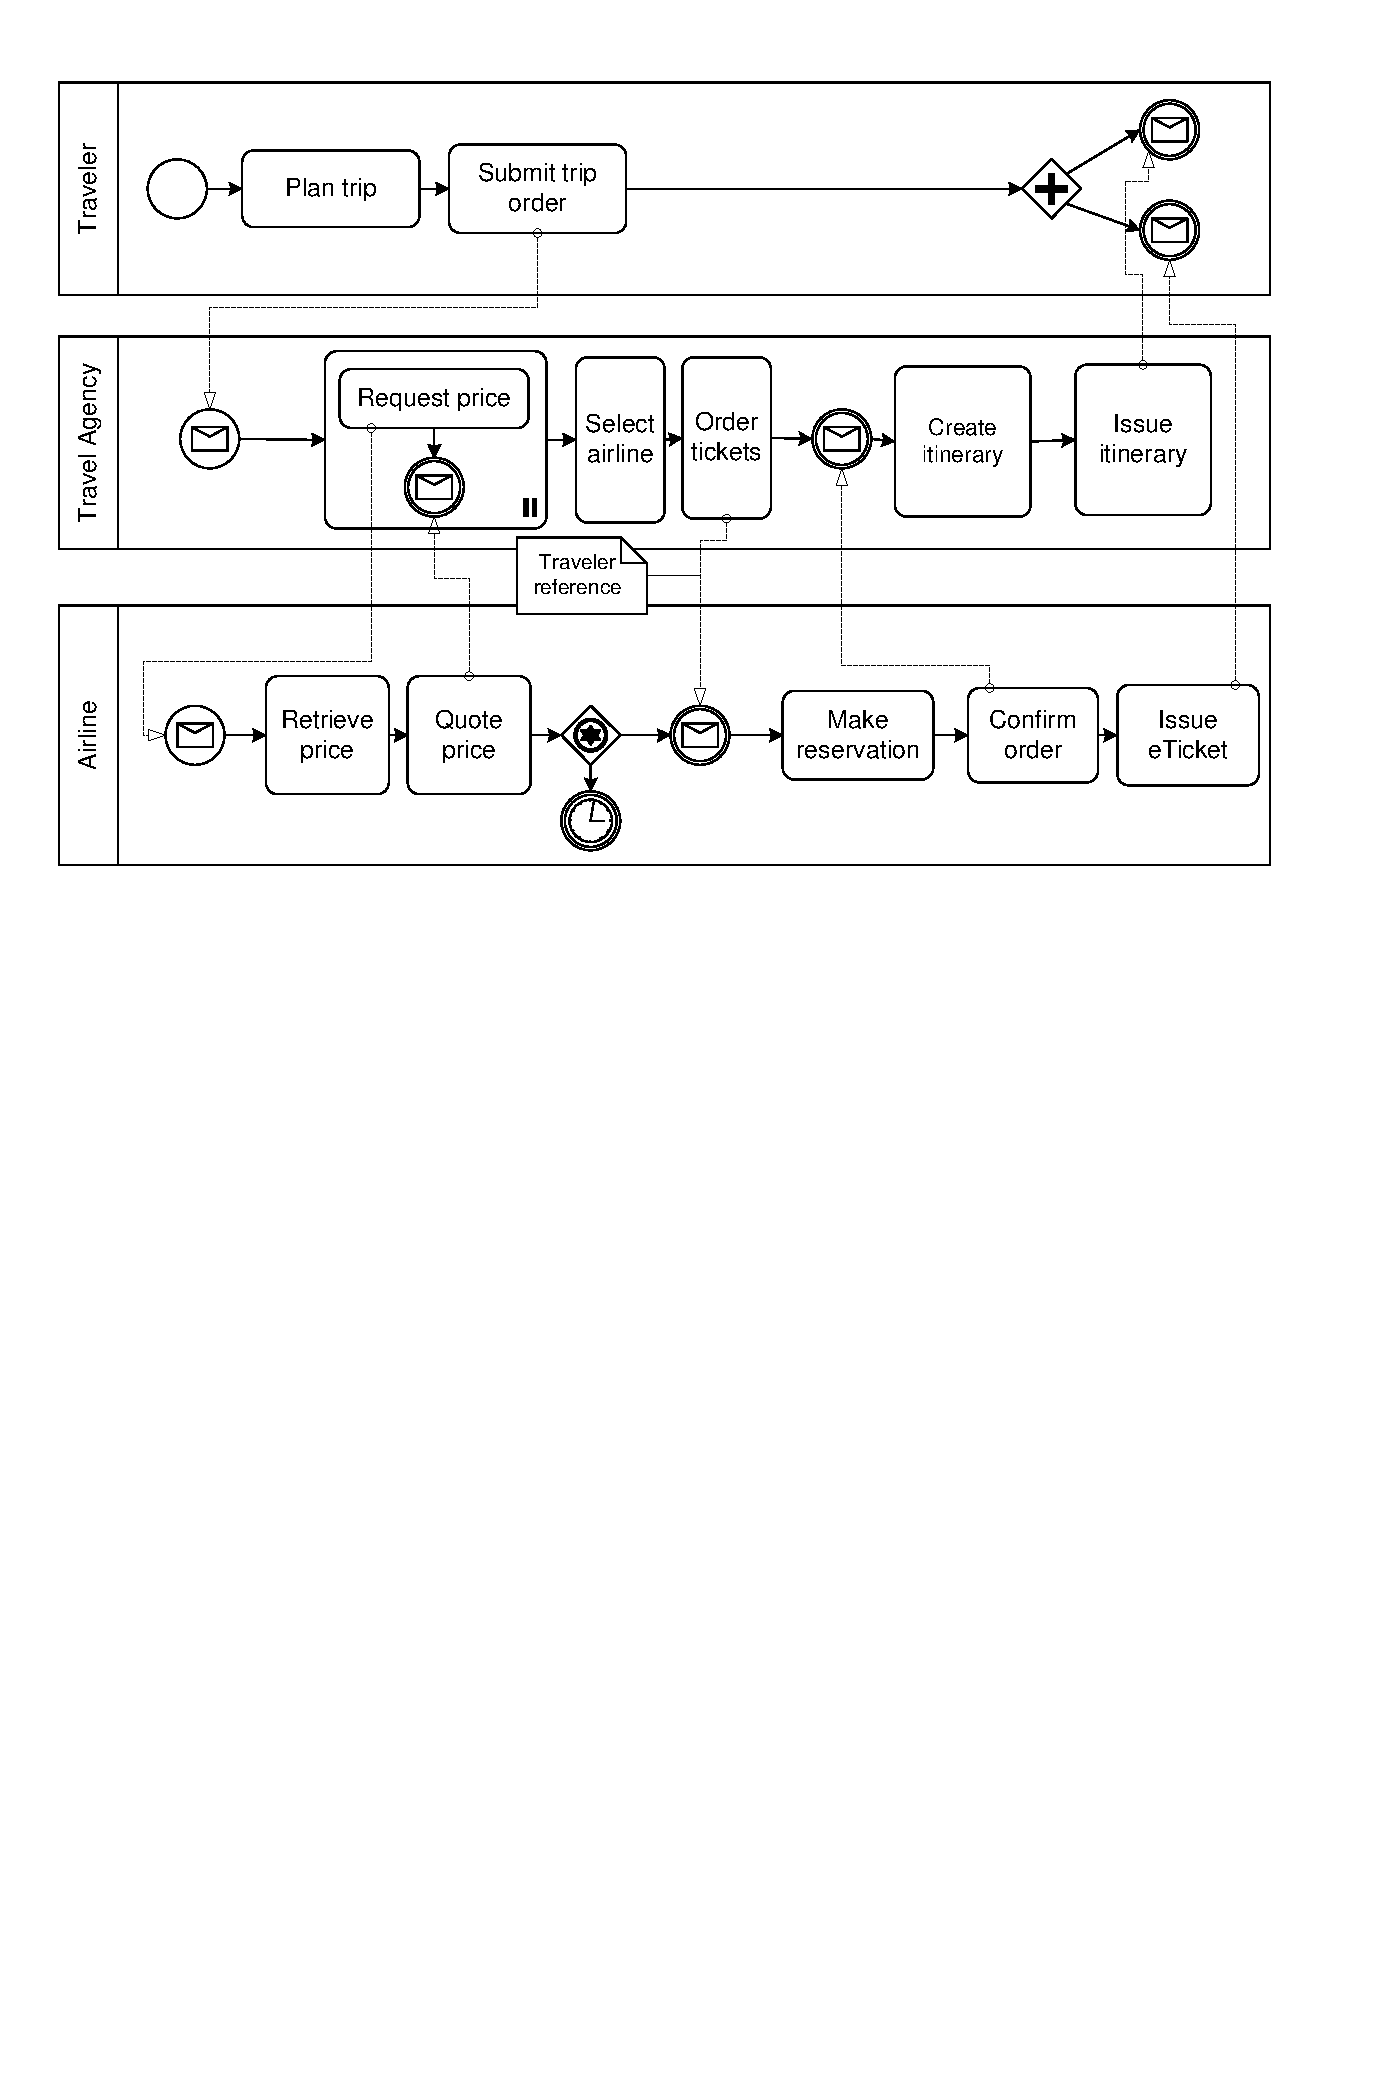
\includegraphics[width=\textwidth]{choreography.pdf}
  \caption{Beispiel-Choreographie}
  \label{fig:chor1}
\end{figure}

\begin{figure}
  \centering
  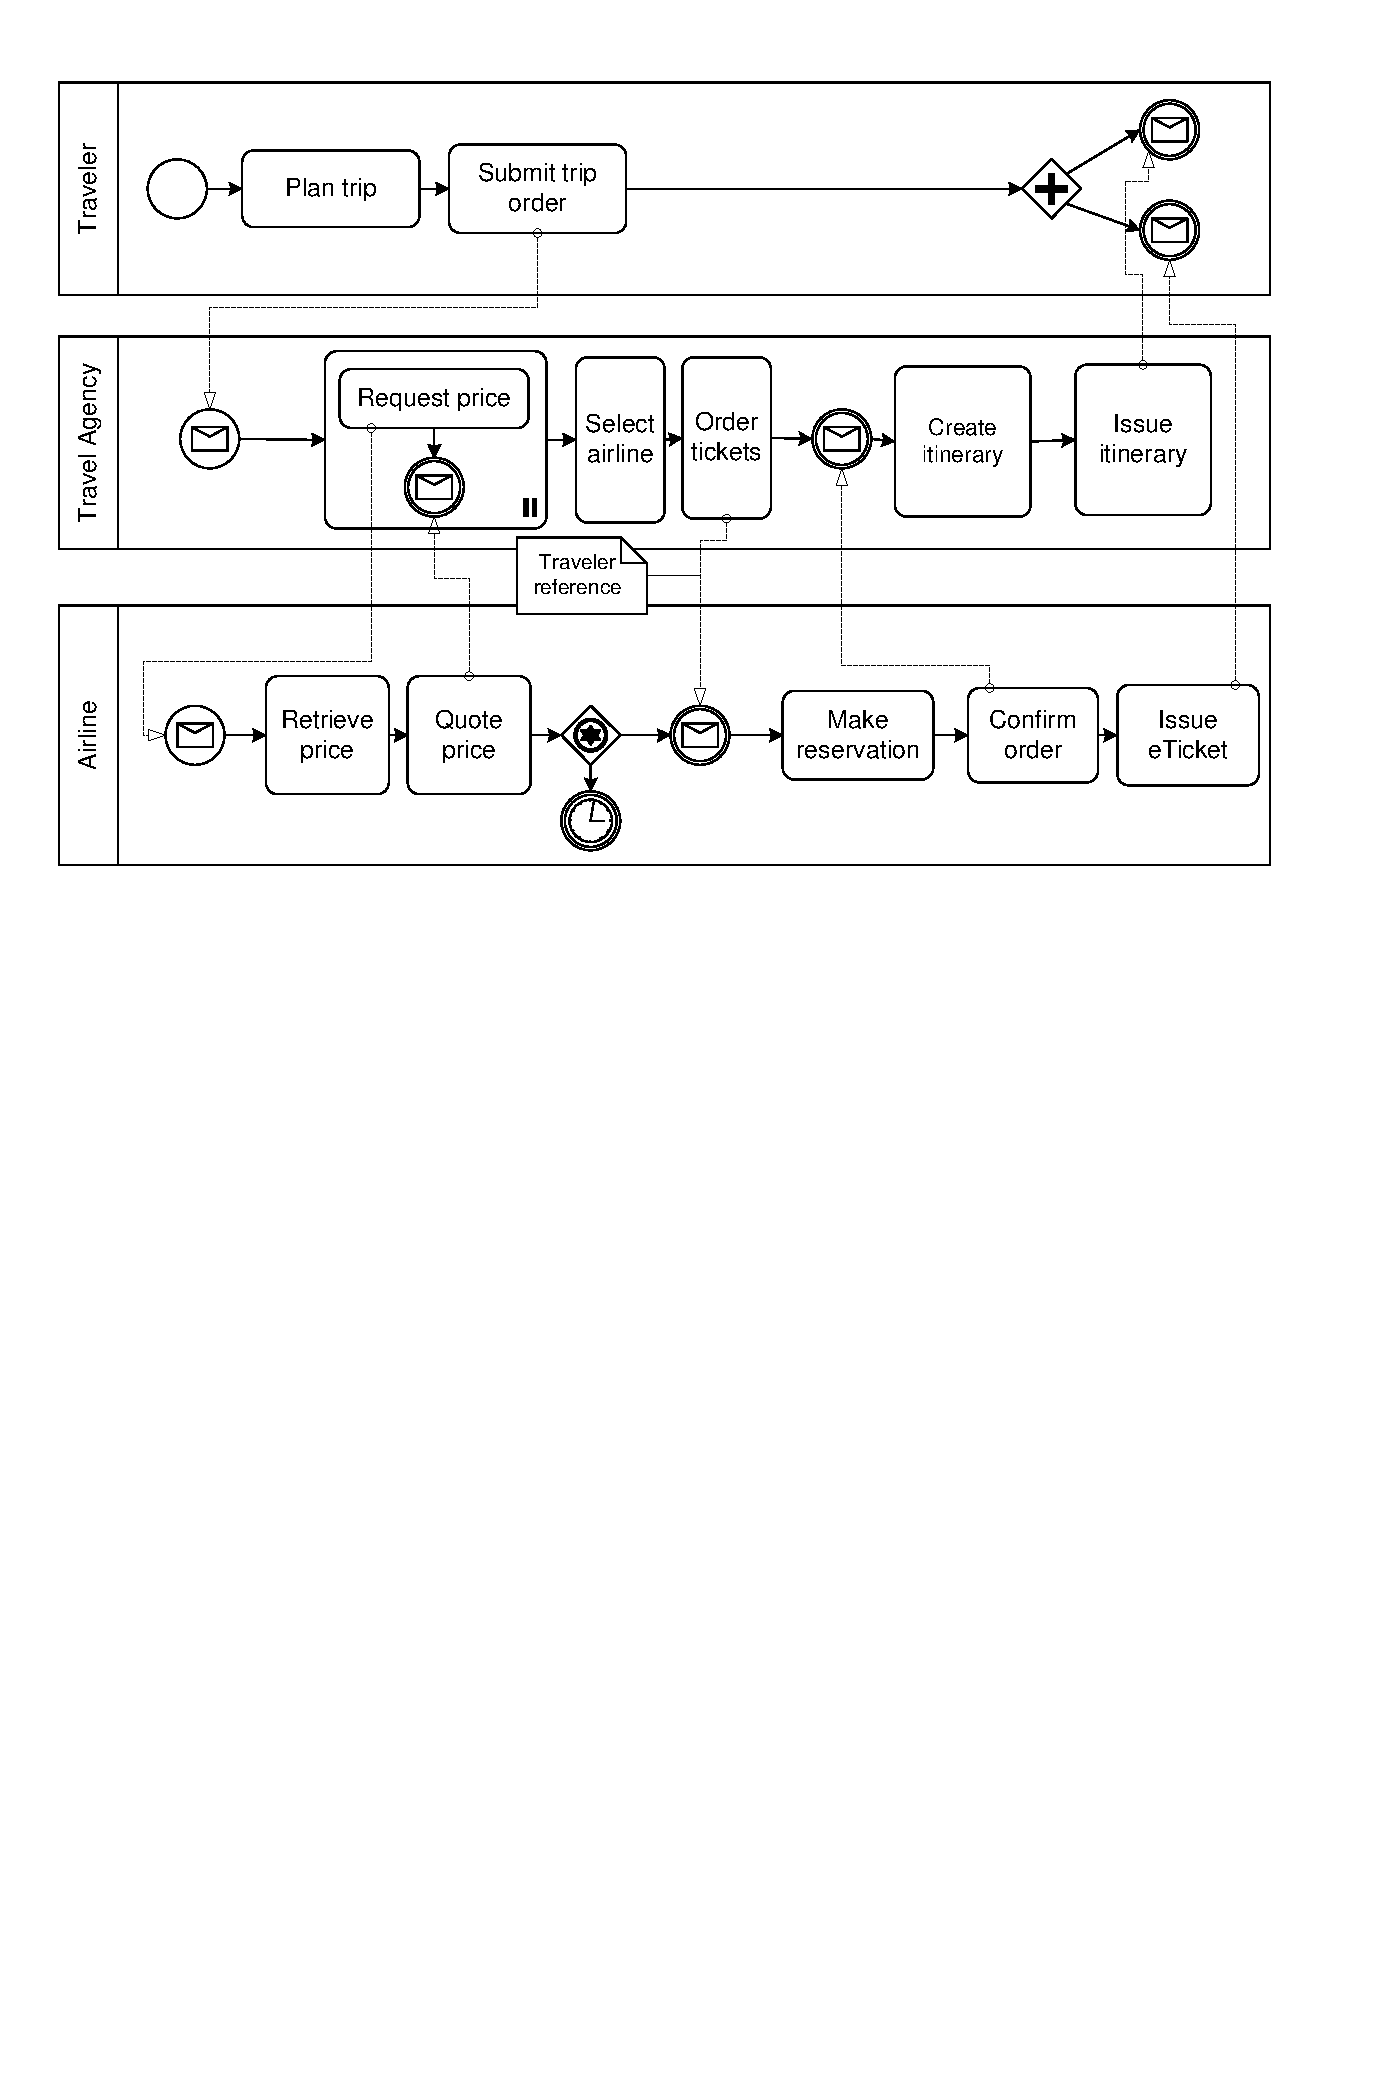
\includegraphics[width=.8\textwidth]{choreography.pdf}
  \caption[Beispiel-Choreographie]{Die Beispiel-Choreographie.
    Nun etwas kleiner, damit \texttt{\textbackslash textwidth} demonstriert wird.
    Und auch die Verwendung von alternativen Bildunterschriften für das Verzeichnis der Abbildungen.
    Letzteres ist allerdings nur Bedingt zu empfehlen, denn wer liest schon so viel Text unter einem Bild?
    Oder ist es einfach nur Stilsache?
  }
  \label{fig:chor2}
\end{figure}


\begin{figure}
  \hfill
  \begin{subfigure}{.3\textwidth}
    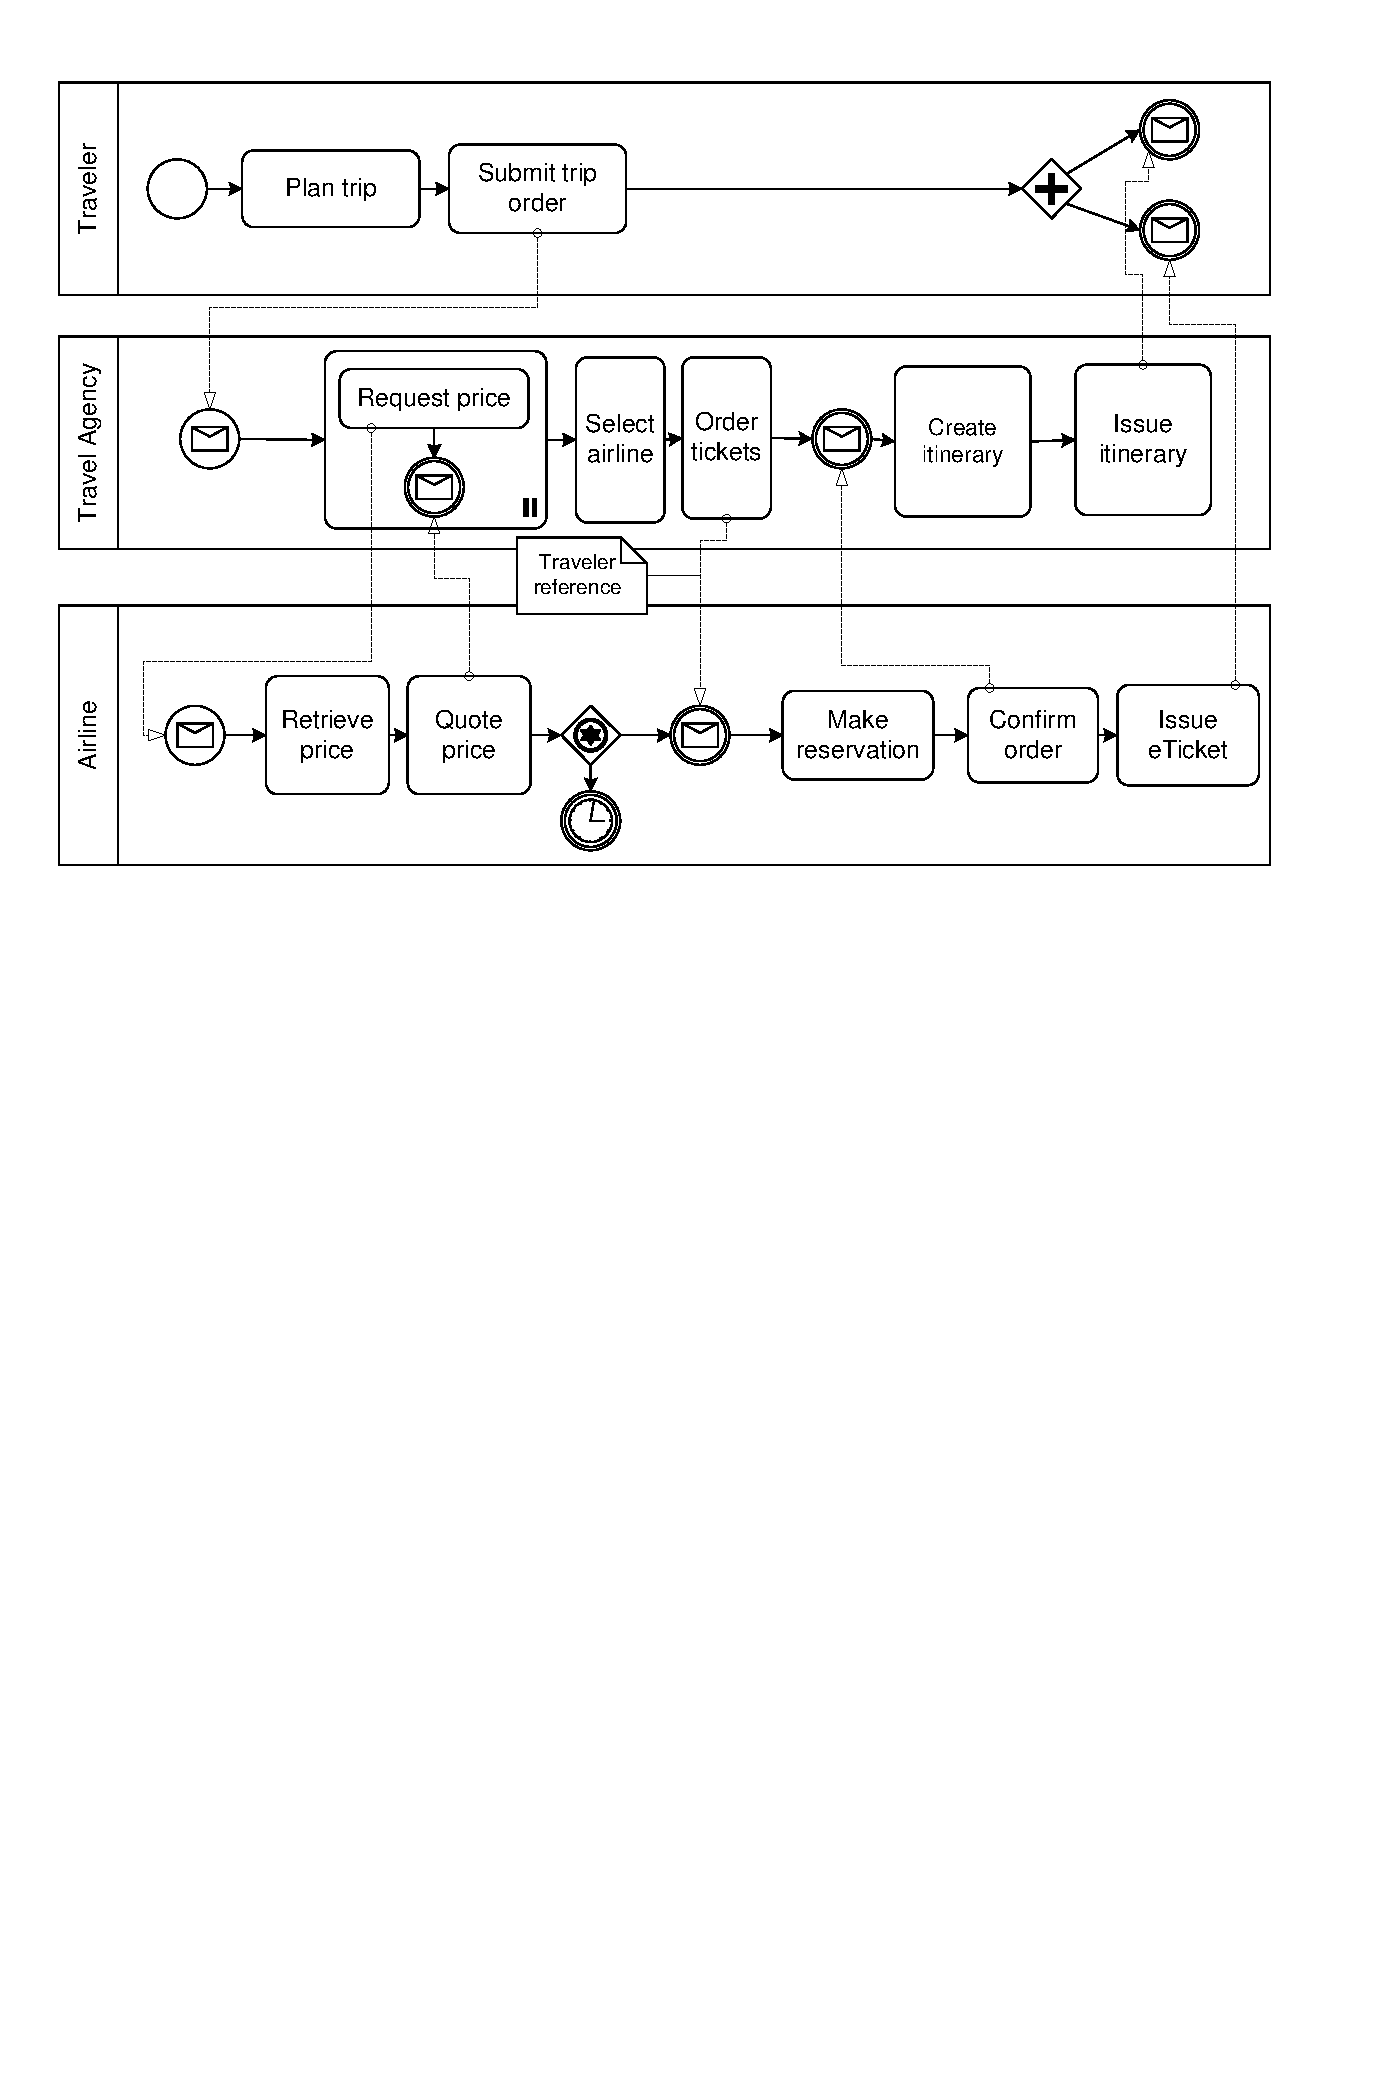
\includegraphics[width=\textwidth]{choreography.pdf}
    \caption{Choreografie 1}
    \label{fig:subfigA}
  \end{subfigure}
  \hfill
  \begin{subfigure}{.3\textwidth}
    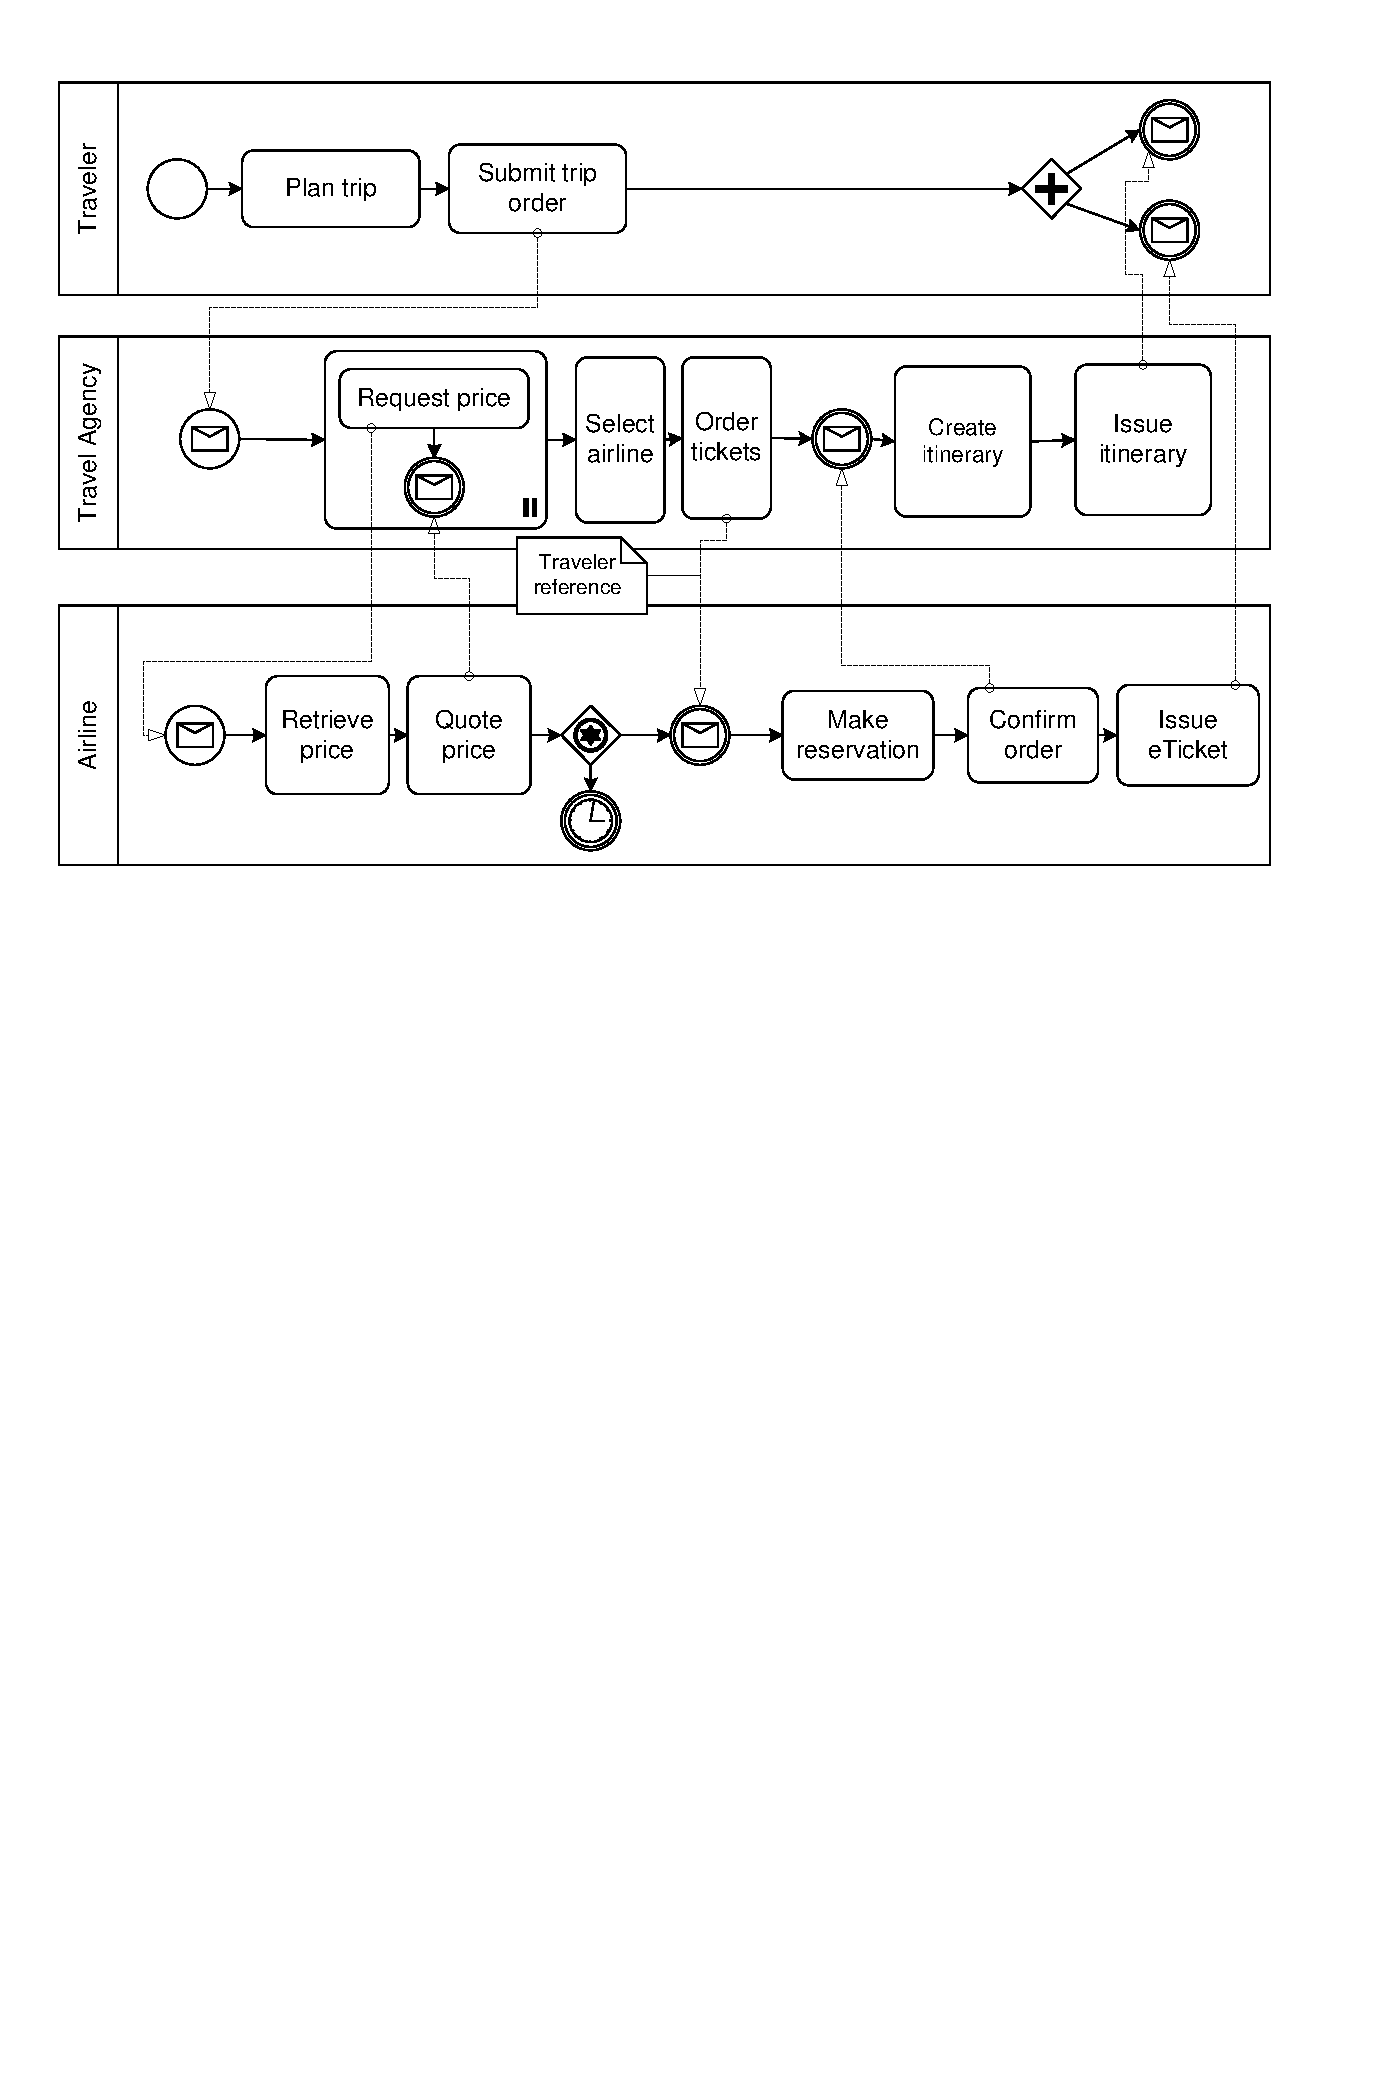
\includegraphics[width=\textwidth]{choreography.pdf}
    \caption{Choreografie 2}
    \label{fig:subfigB}
  \end{subfigure}
  \hfill
  \begin{subfigure}{.3\textwidth}
    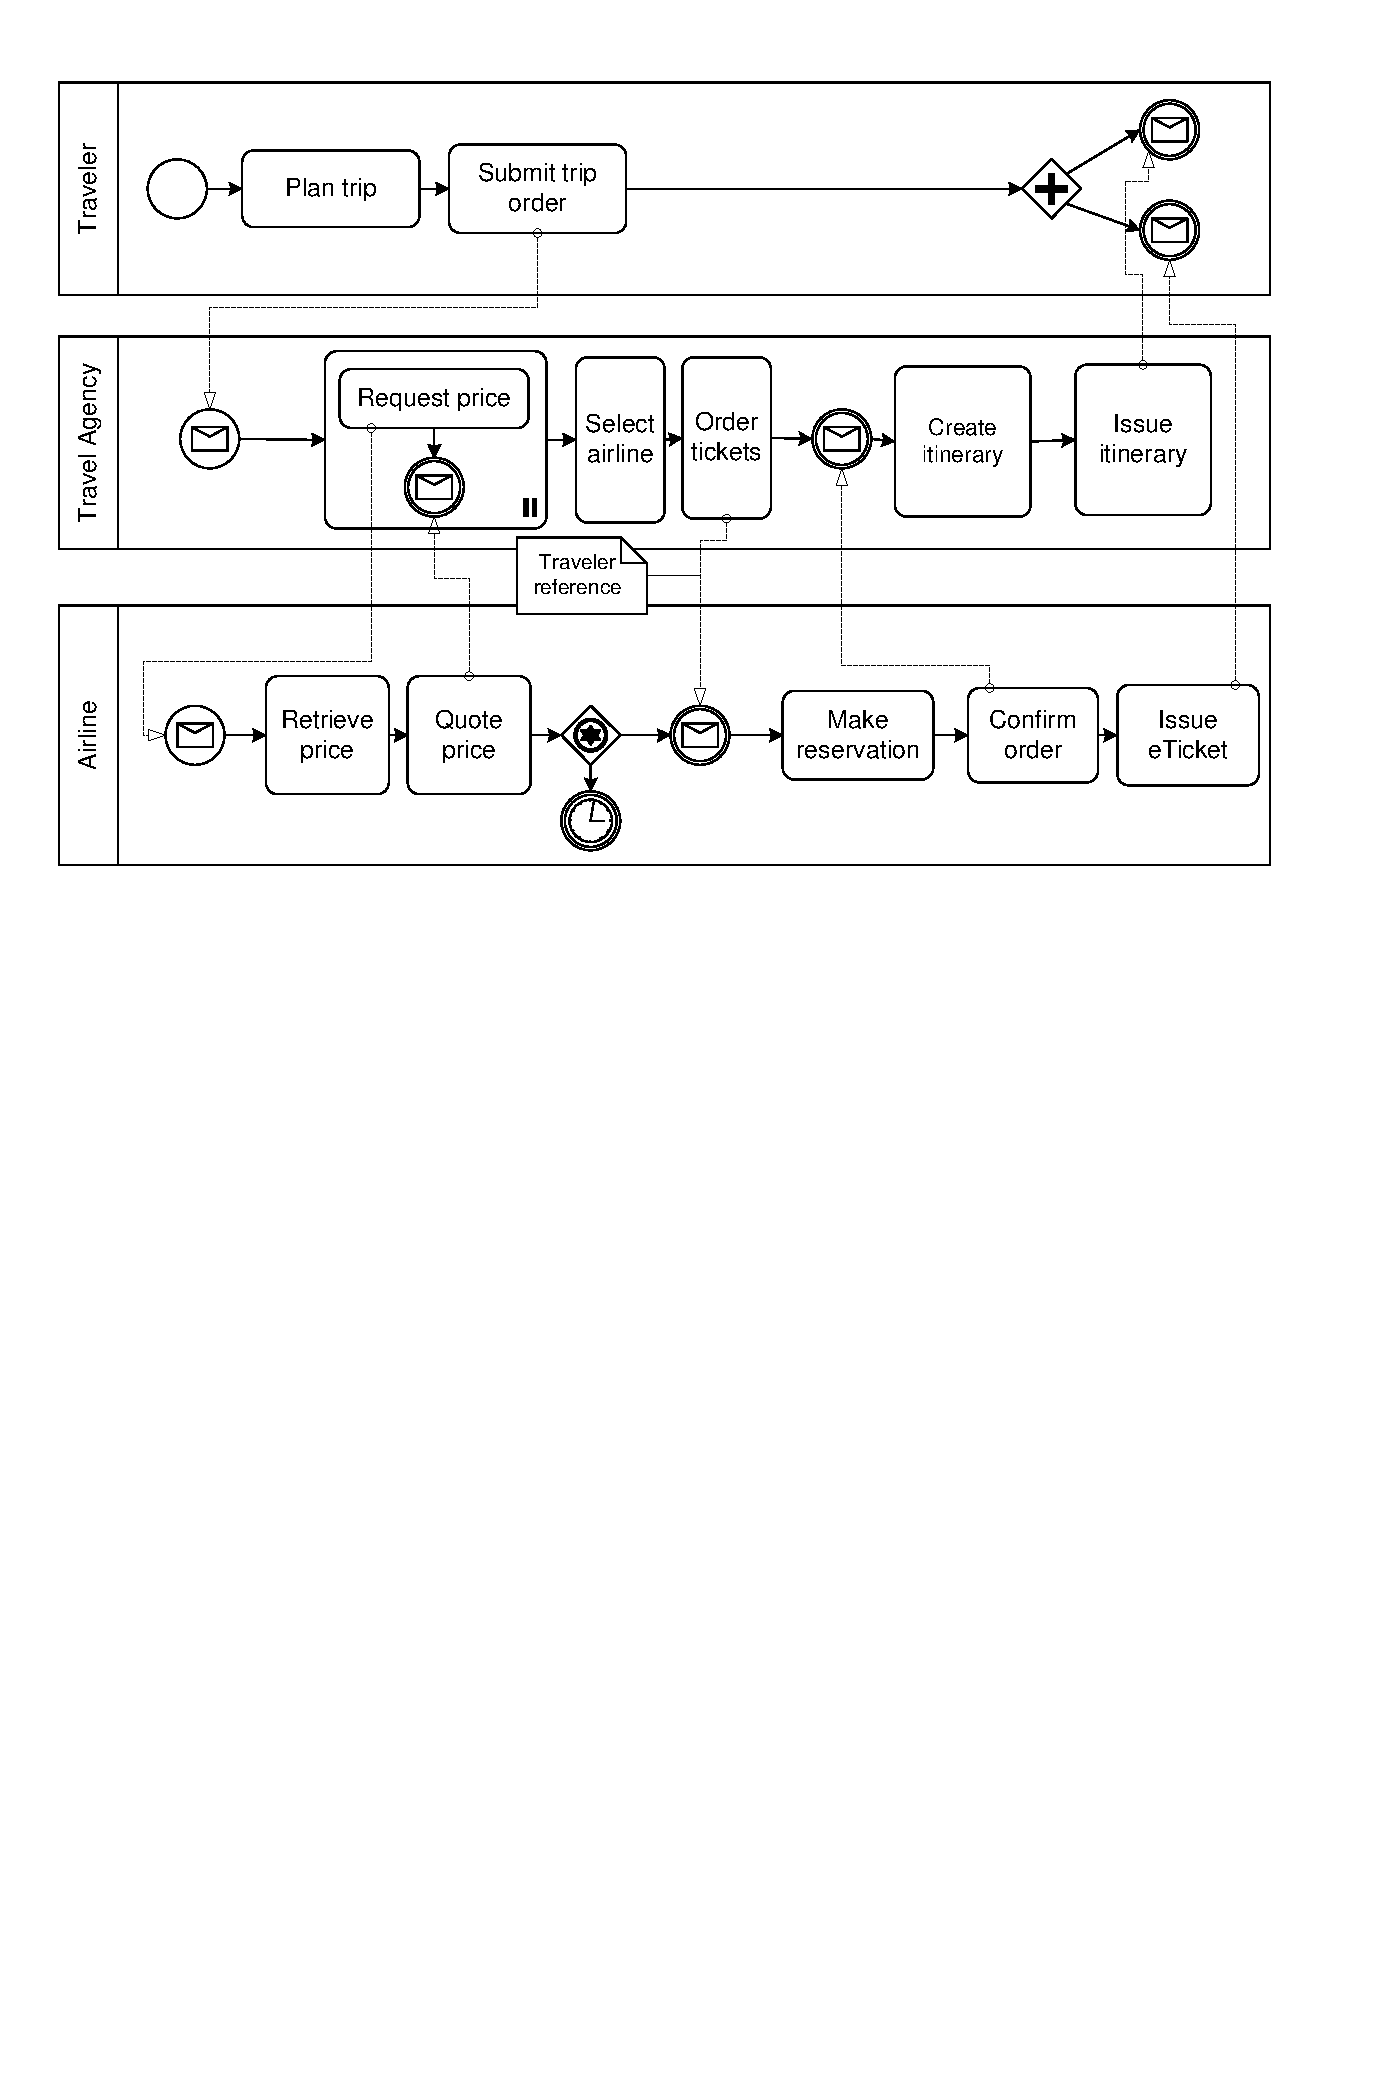
\includegraphics[width=.9\textwidth]{choreography.pdf}
    \caption{Choreografie 3}
    \label{fig:subfigC}
  \end{subfigure}
  \caption{Beispiel um 3 Abbildung nebeneinader zu stellen nur jedes einzeln referenzieren zu können.}
  \label{fig:subfig_example}
\end{figure}

\Cref{fig:subfig_example} zeigt die Verwendung des subcaption-Pakets.
Es ist auch möglich, auf Unterabbildungen zu verweisen: \Cref{fig:subfigA}.

Es ist möglich, SVGs direkt beim Kompilieren in PDF umzuwandeln.
Dies ist im Quellcode zu latex-tipps.tex beschrieben, allerdings auskommentiert.

\iffalse % <-- Das hier wegnehmen, falls inkscape im Pfad ist
  Das SVG in \cref{fig:directSVG} ist direkt eingebunden, während der Text im SVG in \cref{fig:latexSVG} mittels pdflatex gesetzt ist.
  Falls man die Graphiken sehen möchte, muss inkscape im PATH sein und im Tex-Quelltext \texttt{\textbackslash{}iffalse} und \texttt{\textbackslash{}iftrue} auskommentiert sein.

  \begin{figure}
    \centering
    
\includegraphics{svgexample.svg}
    \caption{SVG direkt eingebunden}
    \label{fig:directSVG}
  \end{figure}

  \begin{figure}
    \centering
    \def\svgwidth{.4\textwidth}
    \includesvg{svgexample}
    \caption{Text im SVG mittels \LaTeX{} gesetzt}
    \label{fig:latexSVG}
  \end{figure}
\fi % <-- Das hier wegnehmen, falls inkscape im Pfad ist

\section{Tabellen}

\cref{tab:Ergebnisse} zeigt Ergebnisse und die \cref{tab:Ergebnisse} zeigt wie numerische Daten in einer Tabelle representiert werden können.
\begin{table}
  \centering
  \begin{tabular}{ccc}
    \toprule
    \multicolumn{2}{c}{\textbf{zusammengefasst}} & \textbf{Titel}                                                          \\ \midrule
    Tabelle                                      & wie                                                           & in      \\
    \url{tabsatz.pdf}                            & empfohlen                                                     & gesetzt \\

    \multirow{2}{*}{Beispiel}                    & \multicolumn{2}{c}{ein schönes Beispiel}                                \\
                                                 & \multicolumn{2}{c}{für die Verwendung von \enquote{multirow}}           \\
    \bottomrule
  \end{tabular}
  \caption[Beispieltabelle]{Beispieltabelle -- siehe \url{http://www.ctan.org/tex-archive/info/german/tabsatz/}}
  \label{tab:Ergebnisse}
\end{table}

\begin{table}
  \centering
  \begin{tabular}{l *{8}{d{3.2}}}
    \toprule

                         & \multicolumn{2}{c}{\textbf{Parameter 1}} & \multicolumn{2}{c}{\textbf{Parameter 2}} & \multicolumn{2}{c}{\textbf{Parameter 3}} & \multicolumn{2}{c}{\textbf{Parameter 4}}                                                                                                                                       \\
    \cmidrule(r){2-3}\cmidrule(lr){4-5}\cmidrule(lr){6-7}\cmidrule(l){8-9}

    \textbf{Bedingungen} & \multicolumn{1}{c}{\textbf{M}}           & \multicolumn{1}{c}{\textbf{SD}}          & \multicolumn{1}{c}{\textbf{M}}           & \multicolumn{1}{c}{\textbf{SD}}          & \multicolumn{1}{c}{\textbf{M}} & \multicolumn{1}{c}{\textbf{SD}} & \multicolumn{1}{c}{\textbf{M}} & \multicolumn{1}{c}{\textbf{SD}} \\
    \midrule

    W                    & 1.1                                      & 5.55                                     & 6.66                                     & .01                                      &                                &                                 &                                &                                 \\
    X                    & 22.22                                    & 0.0                                      & 77.5                                     & .1                                       &                                &                                 &                                &                                 \\
    Y                    & 333.3                                    & .1                                       & 11.11                                    & .05                                      &                                &                                 &                                &                                 \\
    Z                    & 4444.44                                  & 77.77                                    & 14.06                                    & .3                                       &                                &                                 &                                &                                 \\
    \bottomrule
  \end{tabular}

  \caption{Beispieltabelle f\"{u}r 4 Bedingungen (W-Z) mit jeweils 4 Parameters mit (M und SD).
  Hinweiß: immer die selbe anzahl an Nachkommastellen angeben.
  }
  \label{tab:Werte}
\end{table}

\section{Pseudocode}
\Cref{alg:sample} zeigt einen Beispielalgorithmus.
\begin{Algorithmus} %Die Umgebung nur benutzen, wenn man den Algorithmus ähnlich wie Graphiken von TeX platzieren lassen möchte
  \caption{Sample algorithm}
  \label{alg:sample}
  %EN: This is an environment from the algorithmicx package
  \begin{algorithmic}
    \Procedure{Sample}{$a$,$v_e$}
      \State $\mathsf{parentHandled} \gets (a = \mathsf{process}) \lor \mathsf{visited}(a'), (a',c,a) \in \mathsf{HR}$
      \State \Comment $(a',c'a) \in \mathsf{HR}$ denotes that $a'$ is the parent of $a$
    \If{$\mathsf{parentHandled}\,\land(\mathcal{L}_\mathit{in}(a)=\emptyset\,\lor\,\forall l \in \mathcal{L}_\mathit{in}(a): \mathsf{visited}(l))$}
      \State $\mathsf{visited}(a) \gets \text{true}$
      \State $\mathsf{writes}_\circ(a,v_e) \gets
        \begin{cases}
          \mathsf{joinLinks}(a,v_e)                & \abs{\mathcal{L}_\mathit{in}(a)} > 0 \\
          \mathsf{writes}_\circ(p,v_e)
                                                   & \exists p: (p,c,a) \in \mathsf{HR}   \\
          (\emptyset, \emptyset, \emptyset, false) & \text{otherwise}
        \end{cases}
      $
    \If{$a\in\mathcal{A}_\mathit{basic}$}
      \State \Call{HandleBasicActivity}{$a$,$v_e$}
    \ElsIf{$a\in\mathcal{A}_\mathit{flow}$}
      \State \Call{HandleFlow}{$a$,$v_e$}
    \ElsIf{$a = \mathsf{process}$} \Comment Directly handle the contained activity
      \State \Call{HandleActivity}{$a'$,$v_e$}, $(a,\bot,a') \in \mathsf{HR}$
      \State $\mathsf{writes}_\bullet(a) \gets \mathsf{writes}_\bullet(a')$
    \EndIf
    \ForAll{$l \in \mathcal{L}_\mathit{out}(a)$}
      \State \Call{HandleLink}{$l$,$v_e$}
    \EndFor
    \EndIf
    \EndProcedure
  \end{algorithmic}
\end{Algorithmus}

\clearpage
Und wer einen Algorithmus schreiben möchte, der über mehrere Seiten geht, der kann das nur mit folgendem \textbf{üblen} Hack tun:

{
\begin{minipage}{\textwidth}
  \hrule height .8pt width\textwidth
  \vskip.3em%\vskip\abovecaptionskip\relax
  \stepcounter{Algorithmus}
  \addcontentsline{alg}{Algorithmus}{\protect\numberline{\theAlgorithmus}{\ignorespaces Description \relax}}
  \noindent\textbf{Algorithmus \theAlgorithmus} Description
  %\stepcounter{algorithm}
  %\addcontentsline{alg}{Algorithmus}{\thealgorithm{}\hskip0em Description}
  %\textbf{Algorithmus \thealgorithm} Description
  \vskip.3em%\vskip\belowcaptionskip\relax
  \hrule height .5pt width\textwidth
\end{minipage}
%without the following line, the text is nerer at the rule
\vskip-.3em
%
code goes here\\
test2\\
%
\vskip-.7em
\hrule height .5pt width\textwidth
}


\section{Abkürzungen}

Beim ersten Durchlauf betrug die \gls{fr} 5.
Beim zweiten Durchlauf war die \gls{fr} 3.~Die Pluralform sieht man hier:\ \glspl{er}.
Um zu demonstrieren, wie das Abkürzungsverzeichnis bei längeren Beschreibungstexten aussieht, muss hier noch \glspl{rdbms} erwähnt werden.

Mit \verb+\gls{...}+ können Abkürzungen eingebaut werden, beim ersten Aufrufen wird die lange Form eingesetzt.
Beim wiederholten Verwenden von \verb+\gls{...}+ wird automatisch die kurz Form angezeigt.
Außerdem wird die Abkürzung automatisch in die Abkürzungsliste eingefügt.
Mit \verb+\glspl{...}+ wird die Pluralform verwendet.
Möchte man, dass bei der ersten Verwendung direkt die Kurzform erscheint, so kann man mit \verb+\glsunset{...}+ eine Abkürzung als bereits verwendet markieren.
Das Gegenteil erreicht man mit \verb+\glsreset{...}+.

Definiert werden Abkürzungen in der Datei \textit{content\\ausarbeitung.tex} mithilfe von \verb+\newacronym{...}{...}{...}+.

Mehr Infos unter: \url{http://tug.ctan.org/macros/latex/contrib/glossaries/glossariesbegin.pdf}

\section{Verweise}
Für weit entfernte Abschnitte ist \enquote{varioref} zu empfehlen:
\enquote{Siehe \vref{sec:mf}}.
Das Kommando \texttt{\textbackslash{}vref} funktioniert ähnlich wie \texttt{\textbackslash{}cref} mit dem Unterschied, dass zusätzlich ein Verweis auf die Seite hinzugefügt wird.
\texttt{vref}: \enquote{\vref{sec:firstsectioninlatexhints}}, \texttt{cref}: \enquote{\cref{sec:firstsectioninlatexhints}}, \texttt{ref}: \enquote{\ref{sec:firstsectioninlatexhints}}.

Falls \enquote{varioref} Schwierigkeiten macht, dann kann man stattdessen \enquote{cref} verwenden.
Dies erzeugt auch das Wort \enquote{Abschnitt} automatisch: \cref{sec:mf}.
Das geht auch für Abbildungen usw.
Im Englischen bitte \verb1\Cref{...}1 (mit großem \enquote{C} am Anfang) verwenden.


%Mit MiKTeX Installation ab dem 2012-01-16 nicht mehr nötig
%Falls ein Abschnitt länger als eine Seite wird und man mittels \texttt{\textbackslash{}vref} auf eine konkrete Stelle in der Section
%verweisen möchte, dann sollte man \texttt{\textbackslash{}phantomsection} verwenden und dann wird
%auch bei \texttt{vref} die richtige Seite angeben.

%%The link location will be placed on the line below.
%%Tipp von http://en.wikibooks.org/wiki/LaTeX/Labels_and_Cross-referencing#The_hyperref_package_and_.5Cphantomsection
%\phantomsection
%\label{alabel}
%Das Beispiel für \texttt{\textbackslash{}phantomsection} bitte im \LaTeX{}-Quellcode anschauen.

%Hier das Beispiel: Siehe Abschnitt \vref{hack1} und Abschnitt \vref{hack2}.

\section{Definitionen}
\begin{definition}[Title]
  \label{def:def1}
  Definition Text
\end{definition}

\Cref{def:def1} zeigt \ldots

\section{Fußnoten}
Fußnoten können mit dem Befehl \verb+\footnote{...}+ gesetzt werden\footnote{\label{fussnote}Diese Fußnote ist ein Beispiel.
}.
Mehrfache Verwendung von Fußnoten ist möglich indem man zu erst ein Label in der Fußnote setzt \verb+\footnote{\label{...}...}+ und anschließend mittels \verb+\cref{...}+ die Fußnote erneut verwendet\cref{fussnote}.

\section{Verschiedenes}
\label{sec:diff}
\ifdeutsch
  Ziffern (123\,654\,789) werden schön gesetzt.
  Entweder in einer Linie oder als Minuskel-Ziffern.
  Letzteres erreicht man durch den Parameter \texttt{osf} bei dem Paket \texttt{libertine} bzw.\ \texttt{mathpazo} in \texttt{fonts.tex}.
\fi

\begin{compactenum}[I.]
  \item Man kann auch die Nummerierung dank paralist kompakt halten
  \item und auf eine andere Nummerierung umstellen
\end{compactenum}

\section{Weitere Illustrationen}
\Cref{fig:AnhangsChor,fig:AnhangsChor2} zeigen zwei Choreographien, die den Sachverhalt weiter erläutern sollen.
Die zweite Abbildung ist um 90 Grad gedreht, um das Paket \texttt{pdflscape} zu demonstrieren.

\begin{figure}
  \centering
  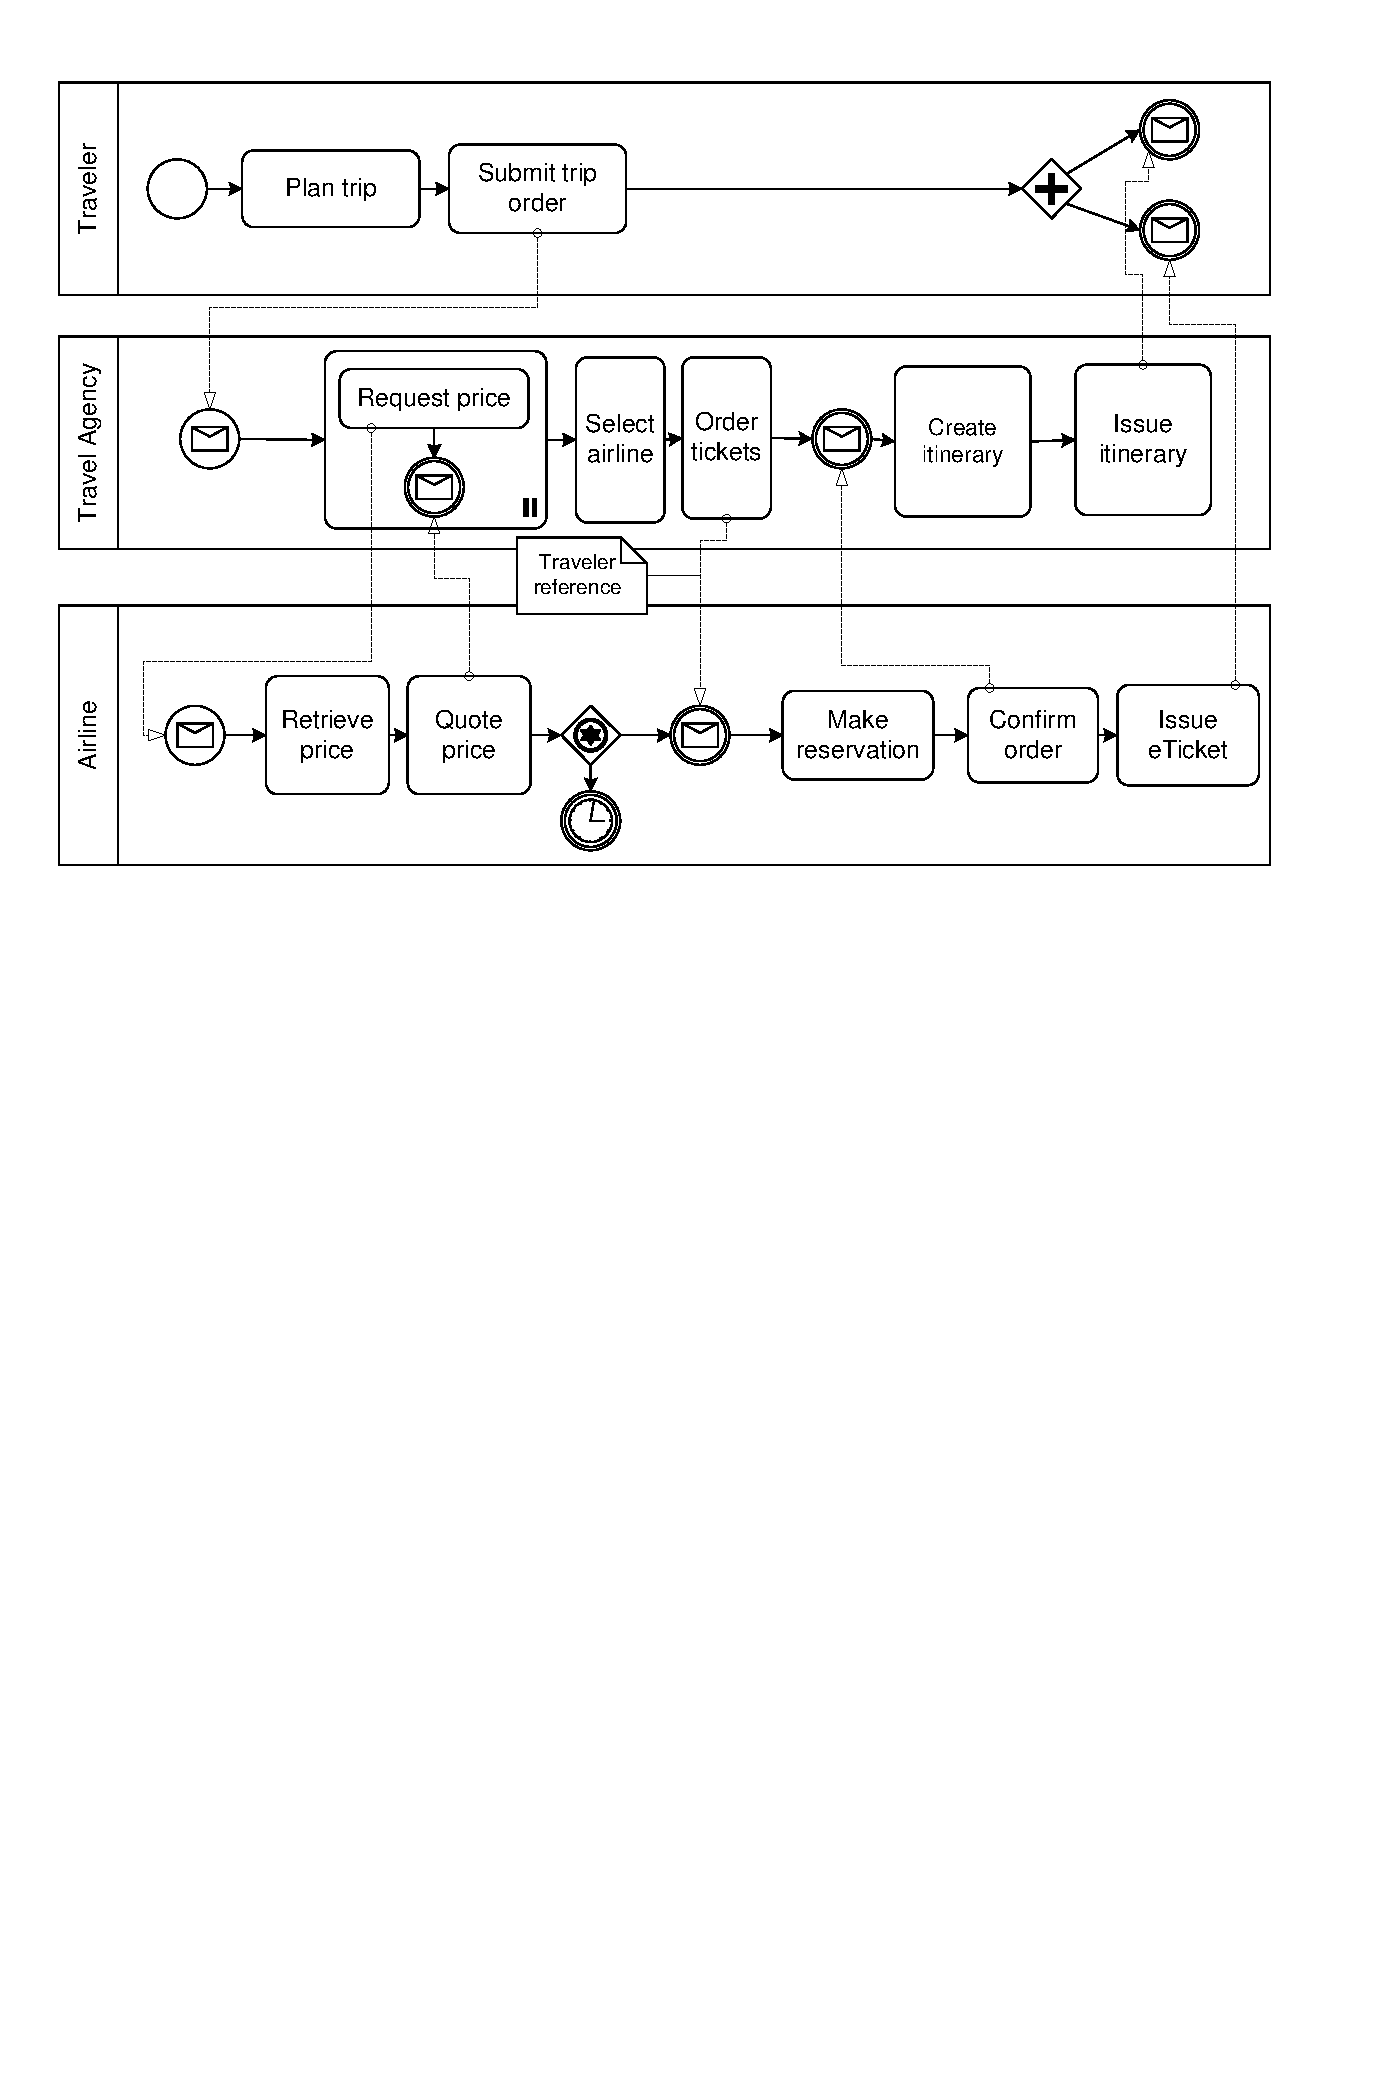
\includegraphics[width=\textwidth]{choreography.pdf}
  \caption{Beispiel-Choreographie I}
  \label{fig:AnhangsChor}
\end{figure}

\begin{landscape}
  \begin{figure}
    \centering
    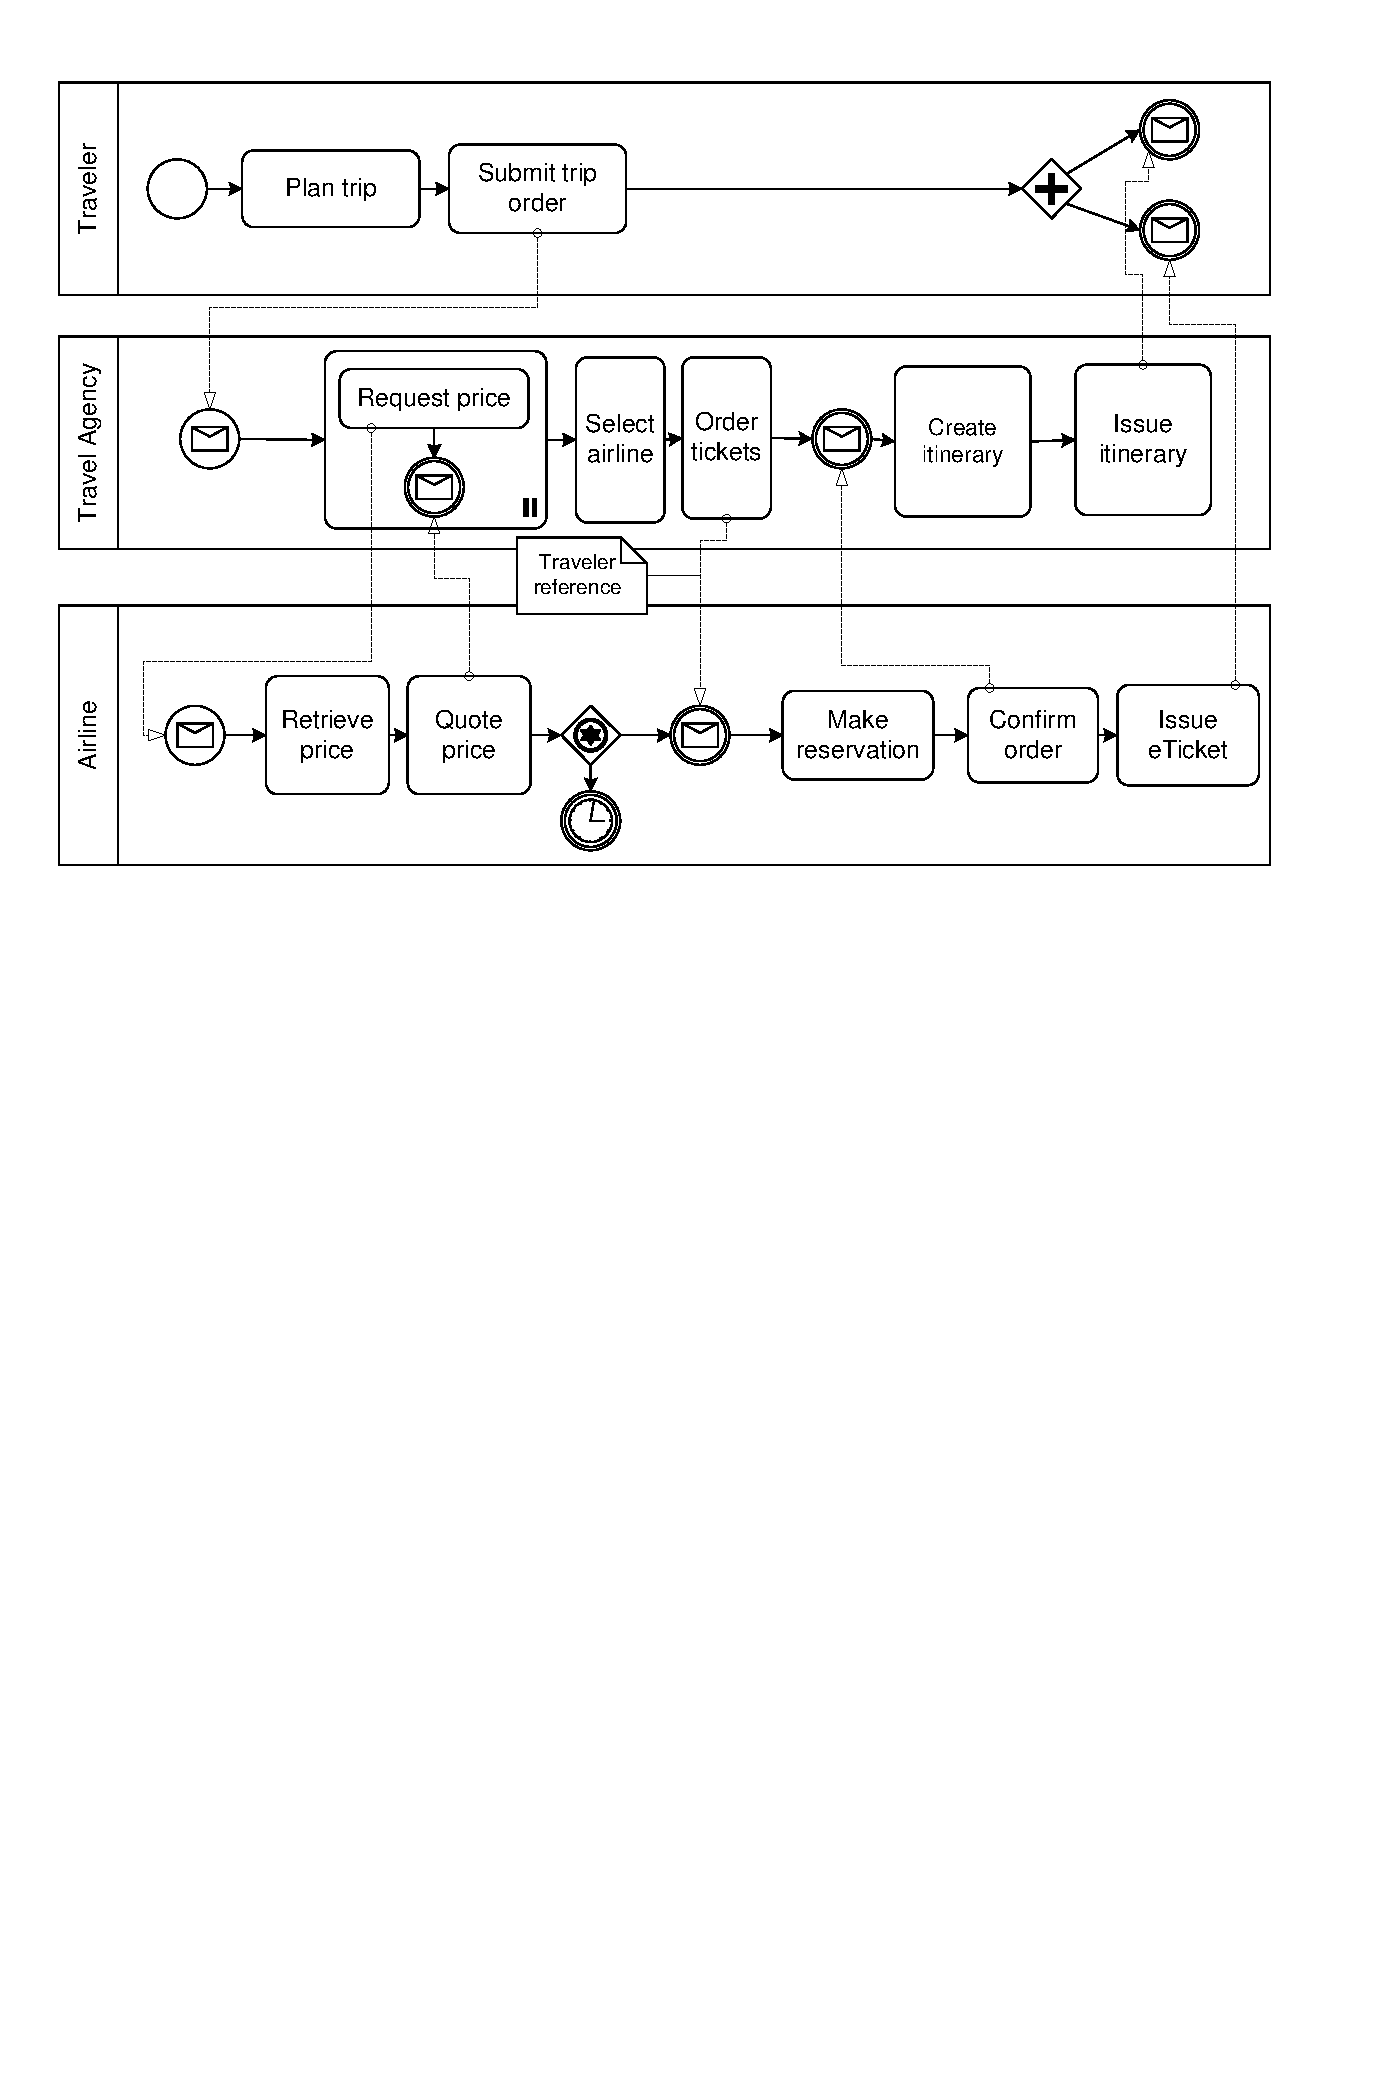
\includegraphics[width=\textwidth]{choreography.pdf}
    \caption{Beispiel-Choreographie II}
    \label{fig:AnhangsChor2}
  \end{figure}
\end{landscape}


\iffalse

  \clearpage

  FIXME - This does not work with MiKTeX as of 2016-12-30

  TODO- demonstrate rotating package

  %hint by http://tex.stackexchange.com/a/3265/9075
  %other option is to use changepage according to http://tex.stackexchange.com/a/2639/9075. This, however, has issues with landscape
  \thispagestyle{empty}

  \savegeometry{koma}

  %If you only have height problems, this is not needed at all
  \addtolength{\textwidth}{2cm}
  \addtolength{\evensidemargin}{-1cm}

  \begin{landscape}
    %sidewaysfigure
    \begin{figure}
      \centering
      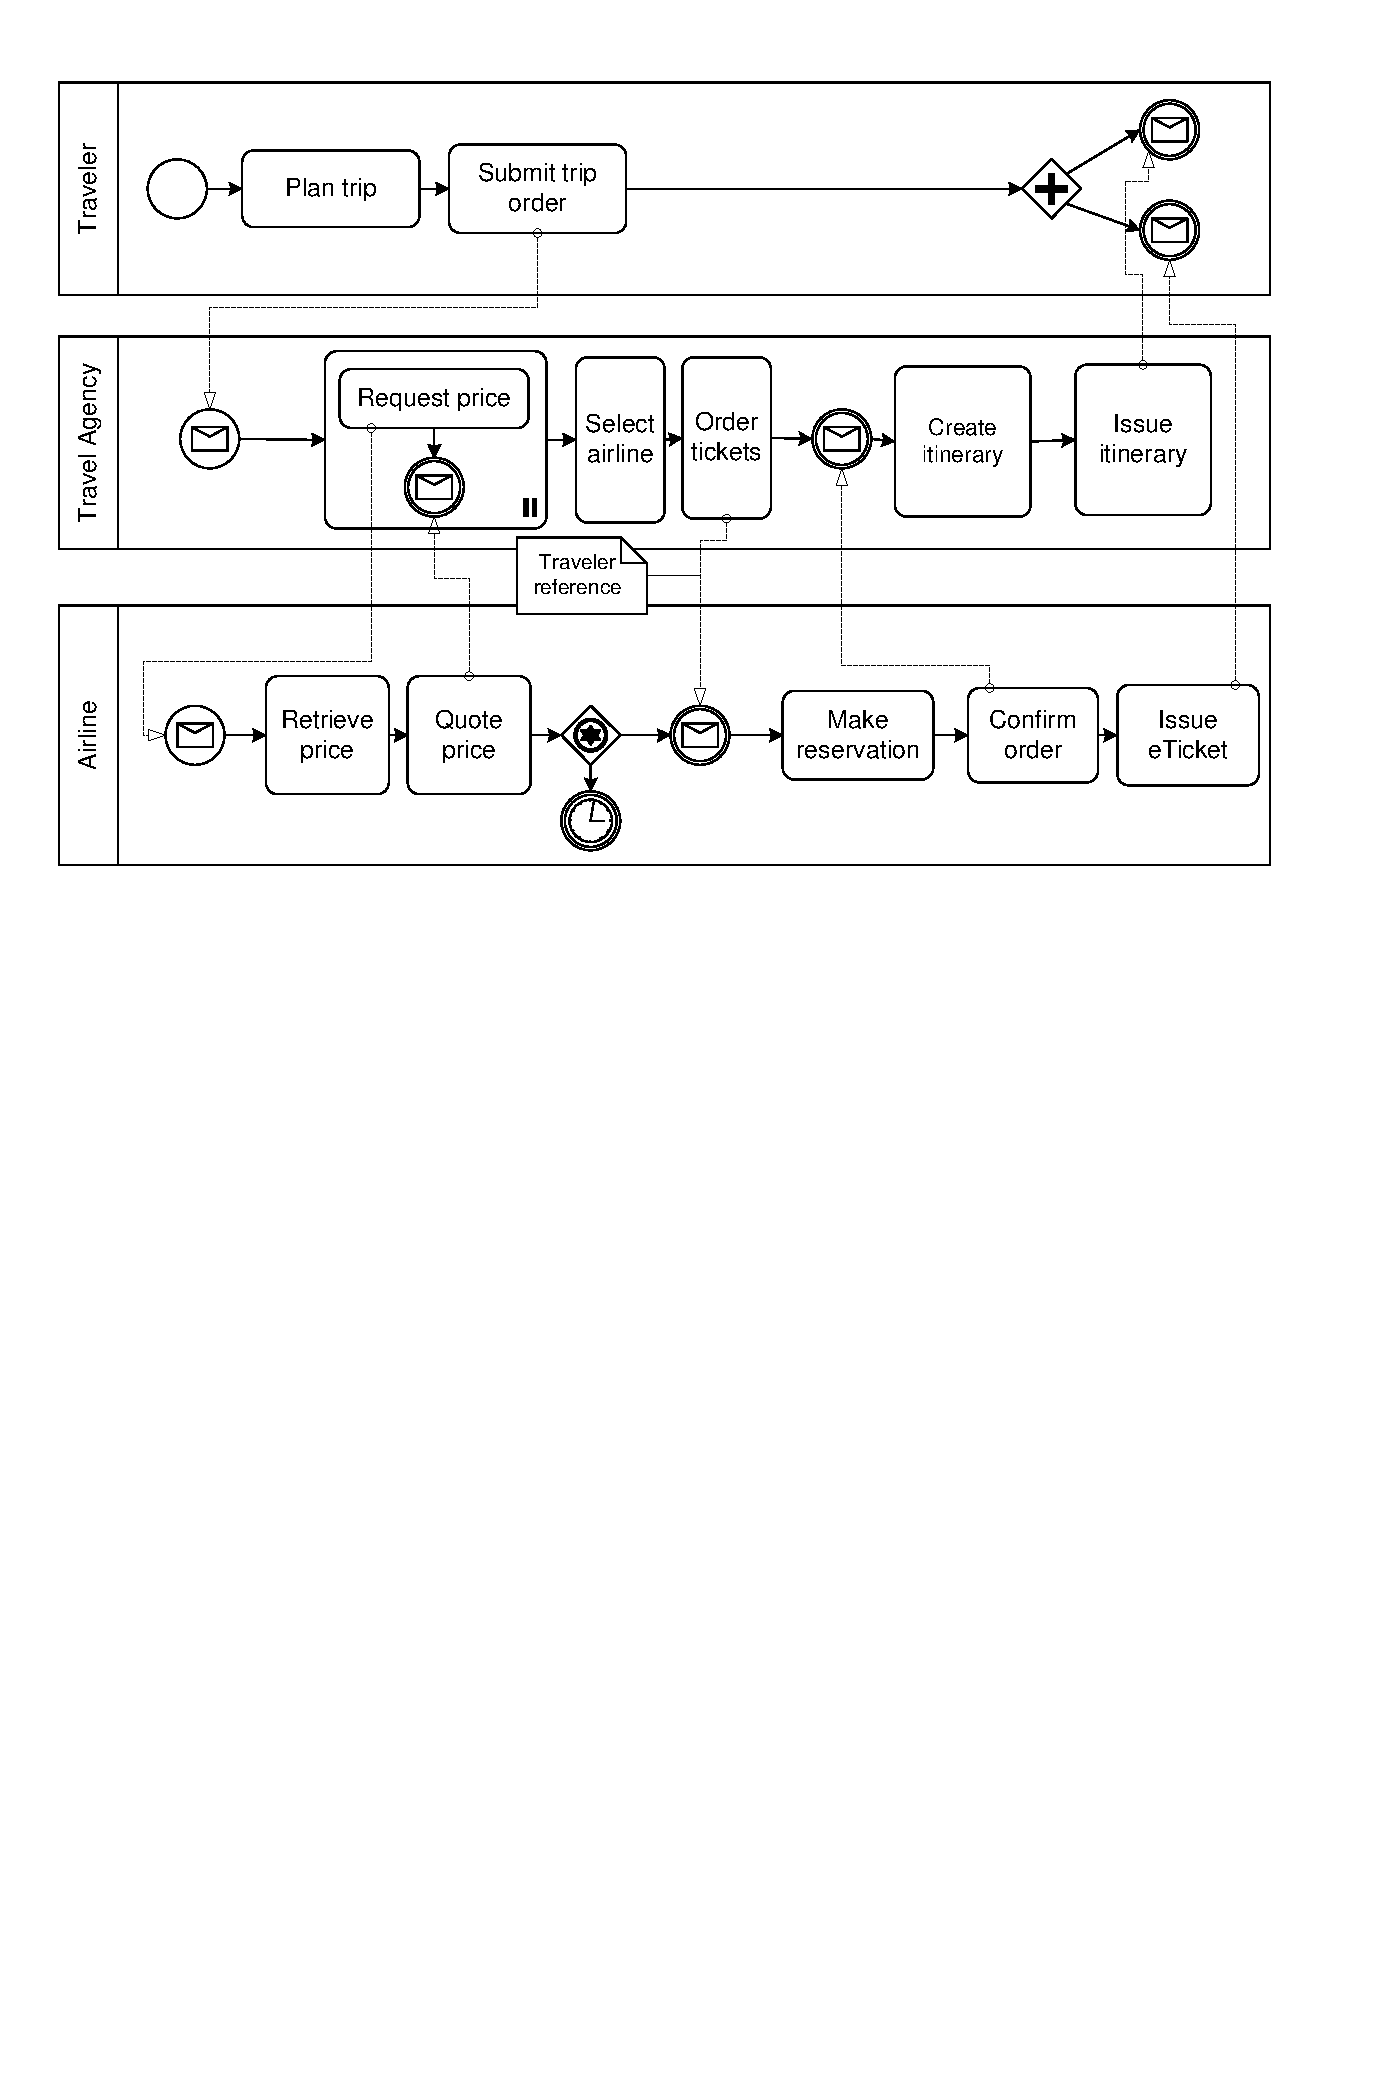
\includegraphics[width=0.9\paperheight]{choreography.pdf}
      \caption{Beispiel-Choreographie, auf einer weißen Seite gezeigt wird und über die definierten Seitenränder herausragt}
    \end{figure}
  \end{landscape}

  %the original layout is restored.
  %%\restoregeometry cannot be used as we use \addtolength
  \loadgeometry{koma}

\fi

\IfFileExists{pgfplots.sty}{
  \section{Plots with pgfplots}
  Pgfplot ist ein Paket um Graphen zu plotten ohne den Umweg über gnuplot oder matplotlib zu gehen.
  %hint by http://tex.stackexchange.com/a/3265/9075%other option is to use changepage according to http://tex.stackexchange.com/a/2639/9075. This, however, has issues with landscape%If you only have height problems, this is not needed at all%sidewaysfigure%the original layout is restored.%%\restoregeometry cannot be used as we use \addtolength
  \begin{figure}[h]
    \begin{center}
      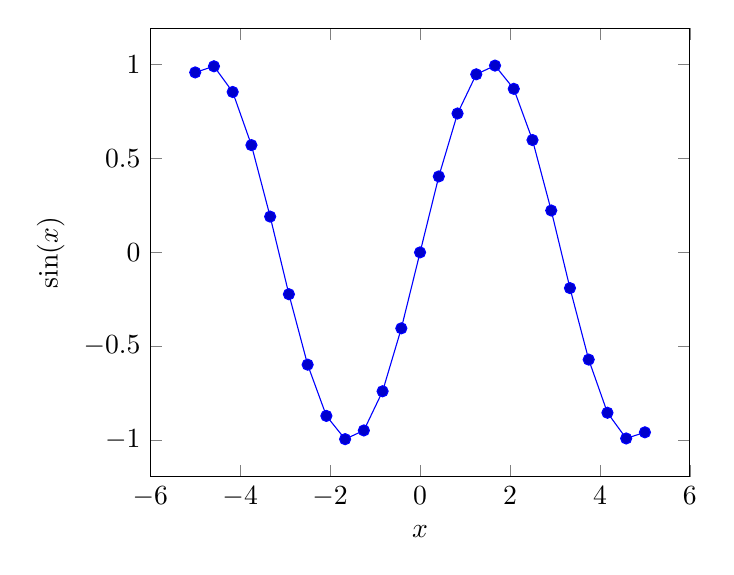
\begin{tikzpicture}
        \begin{axis}[xlabel=$x$,
            ylabel=$\sin(x)$]
          \addplot {sin(deg(x))};  % Sinus-Funktion zeichnen
        \end{axis}
      \end{tikzpicture}
    \end{center}
    \caption{$\sin(x)$ mit pgfplots.}
  \end{figure}
}{}

\IfFileExists{tikz.sty}{
  \section{Figures with tikz}
  TikZ ist ein Paket um Zeichnungen mittels Programmierung zu erstellen.
  Dieses Paket eignet sich um Gitter zu erstellen oder andere regelmäßige Strukturen zu erstellen.
  \begin{figure}[ht]
    \begin{center}
      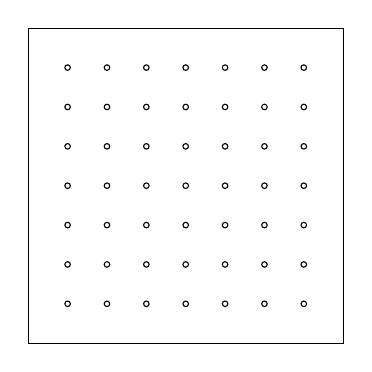
\begin{tikzpicture}
        \draw(0,0) rectangle (4,4);
        \foreach \x in {0.5,1,1.5,2,2.5,3,3.5}
        \foreach \y in {0.5,1,1.5,2,2.5,3,3.5}
        \draw(\x,\y) circle (1pt);
      \end{tikzpicture}
    \end{center}
    \caption{Eine tikz-Graphik.}\label{fig:tikz_example}
  \end{figure}
}{}

\section{Schlusswort}
Verbesserungsvorschläge für diese Vorlage sind immer willkommen.
Bitte bei GitHub ein Ticket eintragen (\url{https://github.com/latextemplates/scientific-thesis-template/issues}).
